\section{Transport}

\begin{itemize}
		\item \SI{10}{\percent} or more packet loss in low-power sensor
				networks due to noisy channels, contention, low signal
				strength, ...
		\item Transport protocols mitigate congestion, recover from packet
				loss, provide error control
		\item Must support self-configuration: Adapt to changing topologies
		\item As well as the usual requirements for low energy usage, ...
		\item Three types: Congestion control, reliability guarantee, TCP-based
				\begin{itemize}
						\item Congestion control optioally with different
								source-to-sink and sink-to-source
								reliabilities.
				\end{itemize}
\end{itemize}

\subsection{Congestion protocols}

\subsubsection{Fusion}

Combines three factors:
\begin{description}
		\item[Hop-by-hop flow control] Congestion bit set dependant on queue
				level. Downstream (further away from sink) nodes seeing
				parent's congestion bit stop forwarding data.
		\item[Prioritized MAC protocol] Smaller back-off window for congested nodes.
		\item[Rate limiting source traffic] Node estimates number of sources
				$n$ routing through its parents, takes care to only send one
				packet every $n$ packets sent by parent (fair share, with e.g.
				tokens).
\end{description}

\subsubsection{Adaptive rate control}

\begin{description}
		\item[Congestion detection] packet loss indicates congestion
		\item[Per-node transmission rate] $p \cdot S$, $S$ application transmission rate, $p \in [0, 1]$
		\item[Capacity] Linear increase of $p$ by $\alpha$ when capacity
		\item[Congestion] Multiplicative decrease of $p$ by $\beta$ when congestion
		\item[Routing vs originating traffic] Optionally different $\alpha$,
				$\beta$ for routing vs originating traffic, to penalize routed
				traffic less during congestion. Eg $\beta' = 1.5 \cdot \beta$,
				$\alpha' = \alpha / (N + 1)$
\end{description}

\subsubsection{Event-to-sink reliable transport}

\begin{itemize}
		\item Sink has desired event frequency
		\item Event reporting rate $f$ on each node, decided upon by sink every time interval
		\item Given observed event reliability $r_i$ and desired event
				reliability $R$, no action of $r_i > R$, otherwise $n_i := r_i
				/ R$, then update $f$ based on $n_i$ and notify nodes.
\end{itemize}

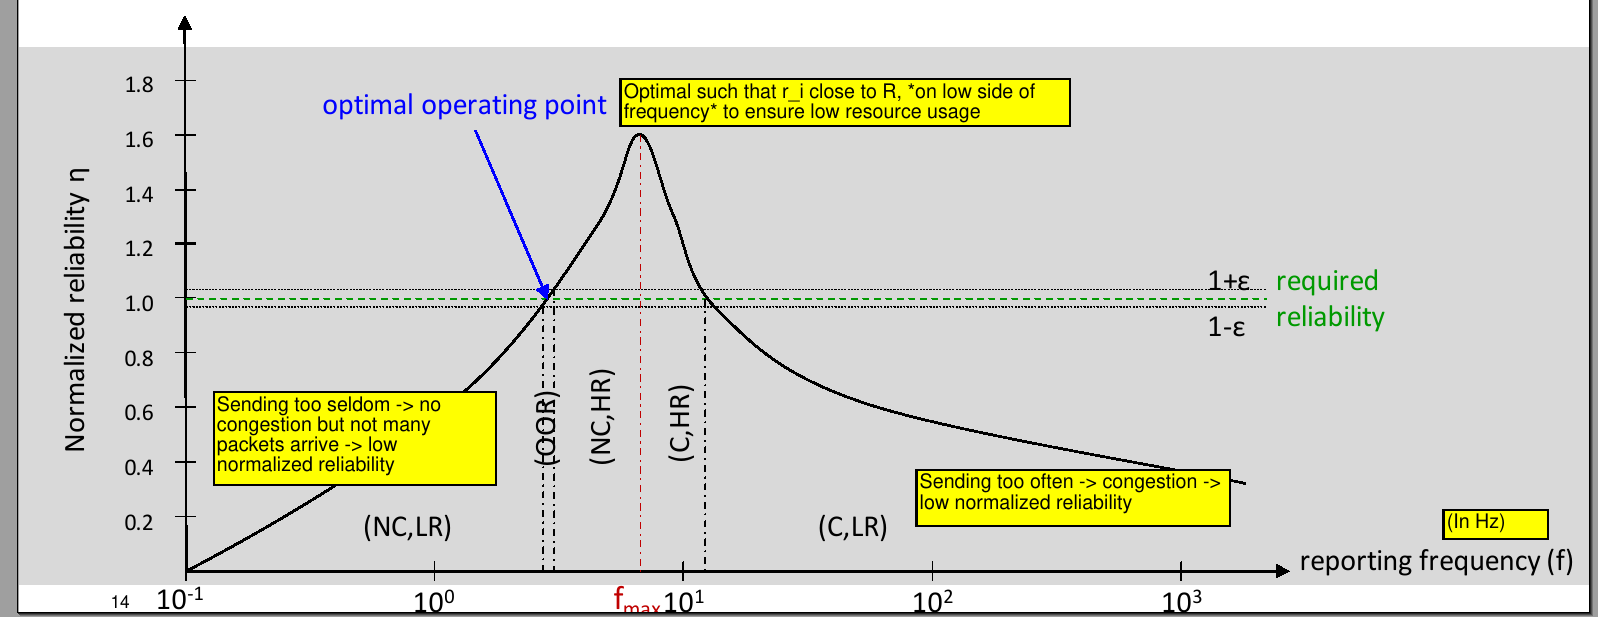
\includegraphics[width=\textwidth]{09_esrt}

\paragraph{Protocol states and actions}

Where NC, C = (No) congestion, LR, HR = Low/High reliability, OOR = optimal operating region.

\begin{description}
		\item[NC, LR] If $f < f_{max}, n < 1 - \epsilon$, then $f_{i+1} := f_{i} / n_i$, multiplicative increase
		\item[NC, HR] If $f \leq f_{max}, n > 1 + \epsilon$, then $f_{i+1} := f_i / 2 \cdot (1 + 1/n_i)$, conservative decrease
		\item[C, HR] If $f > f_{max}, n > 1$, then  $f_{i+1} := f_i / n_i$, aggressive decrease to (NC, HR)
		\item[C, LR] If $f > f_{max}, n \leq 1$, then $f_{i+1} := f_i^{n_i / k}$, exponential decrease where $k$ number of rounds in (C, LR) to decrease congestion
		\item[OOR] If $f < f_{max}, n \in [1 - \epsilon, 1 + \epsilon]$, then $f_{i + 1} := f_i$, no change
\end{description}

\subsubsection{Congestion detection and avoidance, CODA}

\begin{itemize}
		\item Detect congestion by monitoring channel load and buffers
		\item Open-loop backpressure (fast): Nodes broadcast backpressure
				signal during congestion. Source nodes should throttle sending
				rates or drop packets, or forward backpressure.
		\item Closed-loop multi-source regulation (slow): Sink sends feedback
				to specific nodes, regulating their event rate if too many
				events from one source arrive.
\end{itemize}

\subsection{Reliability protocols}

\subsubsection{Reliable Multi-Segment Transport, RMST}

\begin{itemize}
		\item Designed as transport layer for directed diffusion routing
		\item In-network caching
		\item End-to-end reliability, unlike e.g. ESRT
		\item No in-order delivery
\end{itemize}


\paragraph{RMST MAC layer options}

Note: Reliability in MAC layer allows hop-by-hop, which increases chance of
success over many hops compared to reliability in application/transport layer.
RMST uses choice / hybrid solution for MAC layer:

\begin{description}
		\item[No ARQ (automatic repeat request)] All transmissions broadcast,
				no ACK. Reliability deferred to upper layers, no control
				overhead.
		\item[ARQ always] All transmissions unicast, always ACKed. One-to-many
				emulated via multiple unicasts. High probability of packets
				being delivered.
		\item[Selective ARQ] Broadcast for one-to-many, unicast for one-to-one. Data along established paths unicast. Route discover broadcast.
\end{description}

\paragraph{RMST transport layer options}

\begin{description}
		\item[End-to-end selective request NACK] Loss detection at sinks,
				repair requests travel in reverse direction from sink to
				source.
		\item[Hop-by-hop selective request NACK] Each node along path caches
				data, loss detection at each node. Repair request sent to
				immediate neighbour, or to source if neighbours have no
				caching.
\end{description}

\paragraph{RMST application layer options}

\begin{itemize}
		\item Application can either wait for next reading
		\item Or have source send data in fragments, with sink communicating
				interest until all fragments received.
\end{itemize}

\paragraph{Performance results}

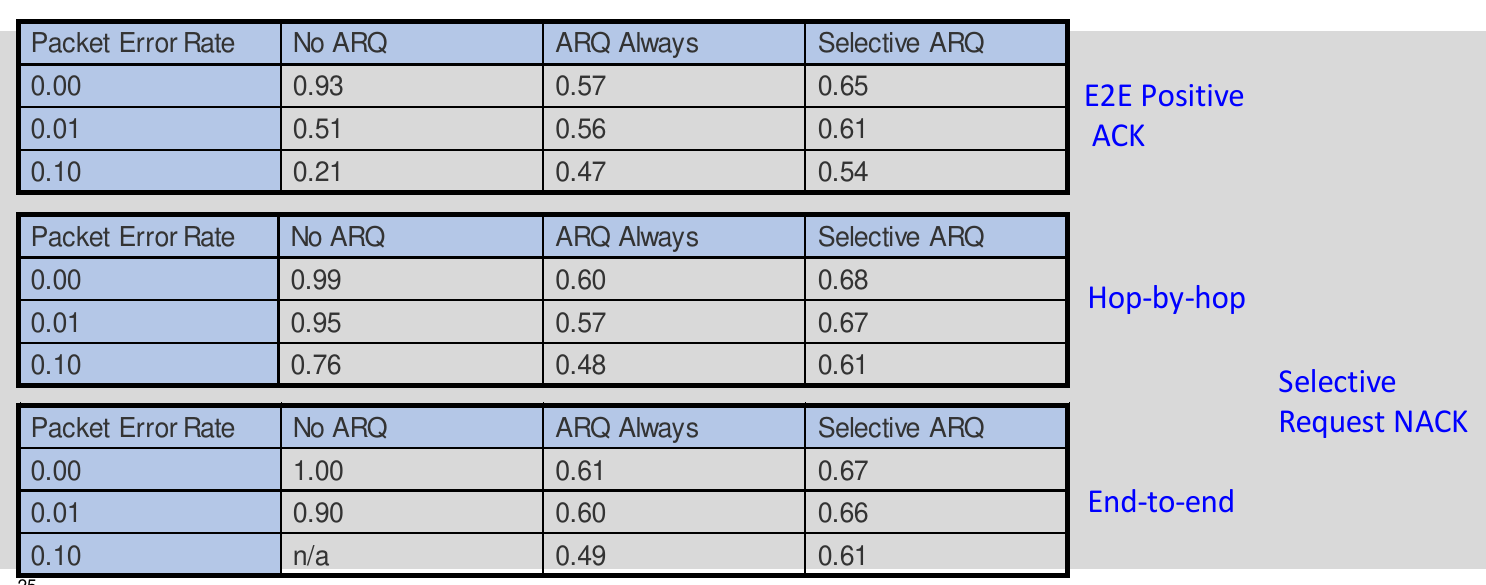
\includegraphics[width=\textwidth]{09_rmst}

\subsubsection{Pump Slowly Fetch Quickly, PSFQ}

\begin{itemize}
		\item Source transmits slowly, to allow intermediate nodes to fetch
				missing segments from neighbour (hop-by-hop recovery). Allows
				local recovery.
		\item Source sends file ID, length, sequence number, TTL and payload.
		\item Node on receiving a chunk decrements TTL, discard if TTL = 0 or
				previously already received it, delays it randomly then
				broadcasts it further.
		\item Node enters fetch mode when sequence gap detected, sends NACK to
				immediate neighbours until gap filled.
		\item Neighbours receiving NACK retransmit after arndom delay.
\end{itemize}

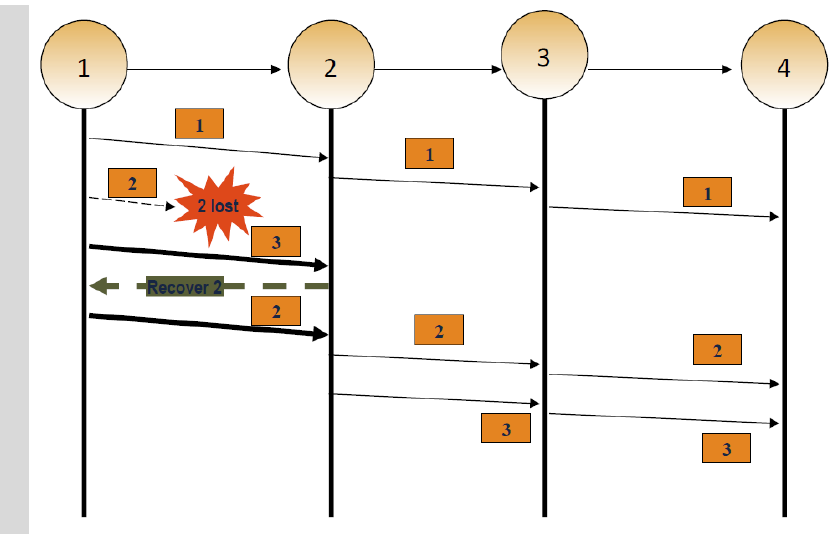
\includegraphics[width=\textwidth]{09_psfq}

\subsection{TCP in IoT}

Problems of not using TCP: Need to translate between transport protocol and TCP
where it's used in the outside world / the sensor network.

Problems of using TCP: Designed for wired internet with poor performance in
wireless network. Does not differentiate congestion and transmission losses.
Does congestion control only in endpoints.

\subsubsection{TCP in uIP}

\begin{itemize}
		\item Statically allocated, single global buffer with only space for one segment
		\item RTT estimation using Karn's algorithm
		\item Retransmission in collaboration with application
\end{itemize}

\subsubsection{Distributed TCP caching}

\begin{itemize}
		\item Use TCP for reliable transfer, e.g. configuration management, updates
		\item Cache transmissions inside network, assume each node able to cache one segment
		\item Each node caches segment with highest segment number with certani probability
\end{itemize}

Important mechanisms:

\begin{description}
		\item[Local retransmission] Timeout-based packet loss detection and \textbf{local} (hop-by-hop) retransmission
		\item[Selective TCP ACK] Ability to ack packet 3 if packet 1, 2 missing. So source must only retransmit 1, 2.
\end{description}

Example of both in action:
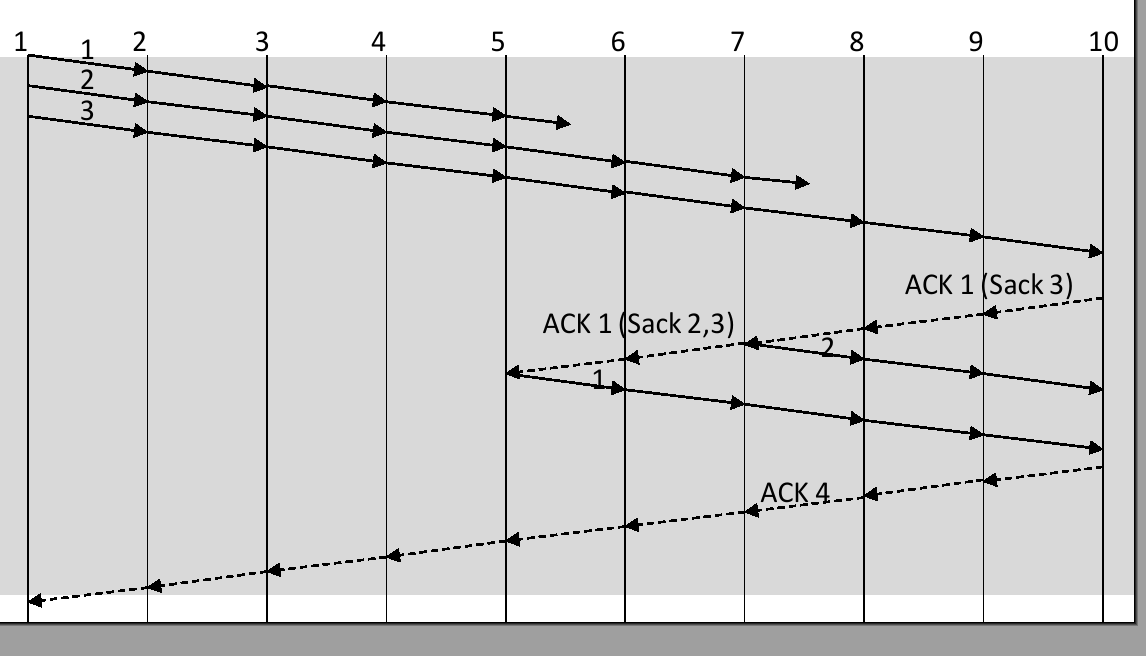
\includegraphics[width=0.5\textwidth]{09_tcp}
